\chapter{Проектирование микросервисной архитектуры с помощью UML диаграмм. }
\textbf{Аннотация.} \textit{Приведено подробное описание спроектированной микросервисной архитектуры с использованием UML диаграмм, демонстрирующих как физическое, так и логическое распределение компонентов. Отражено разделение системы на микросервисы с акцентом на их взаимное взаимодействие через стандартизированные интерфейсы. Приведено описание внешних интерфейсов, обеспечивающих связь с внешними клиентами и другими системами. Отражена модель внутренних интерфейсов, определяющих обмен данными между микросервисами. Приведены UML диаграммы развертывания, иллюстрирующие физическую инфраструктуру, включая использование sidecar-компонентов. Приведены диаграммы последовательности, отражающие все стадии прохождения запросом пути от клиента до сервера и обратно.}




\section{Описание архитектуры системы с помощью диаграммы развертывания.}
\textbf{Аннотация.} \textit{Отражены ключевые аспекты взаимодействия компонентов на основе стандартной UML-нотации. Приведено подробное описание архитектуры системы с разделением на физические и виртуальные узлы. Разработана методика группировки контейнеров в поды для отображения ролей приложений и их sidecar-компонентов. Отражено распределение программных артефактов по физическим серверам и виртуальным машинам в рамках кластера k3s. Приведены зависимости между компонентами, иллюстрирующие потоки данных и сетевые связи. Разработаны схемы, демонстрирующие интеграцию системного мониторинга с помощью fluentbit и Jaeger.Отражены принципы управления трафиком через Istio sidecar для обеспечения безопасности и надежности. Приведено использование Helm-чарта как средства автоматизированного развертывания сервисов. }

(см. рис. \ref{pic:deployment-diagram}).

\begin{figure}[t]
    \centering
    \rotatebox{-90}{%
      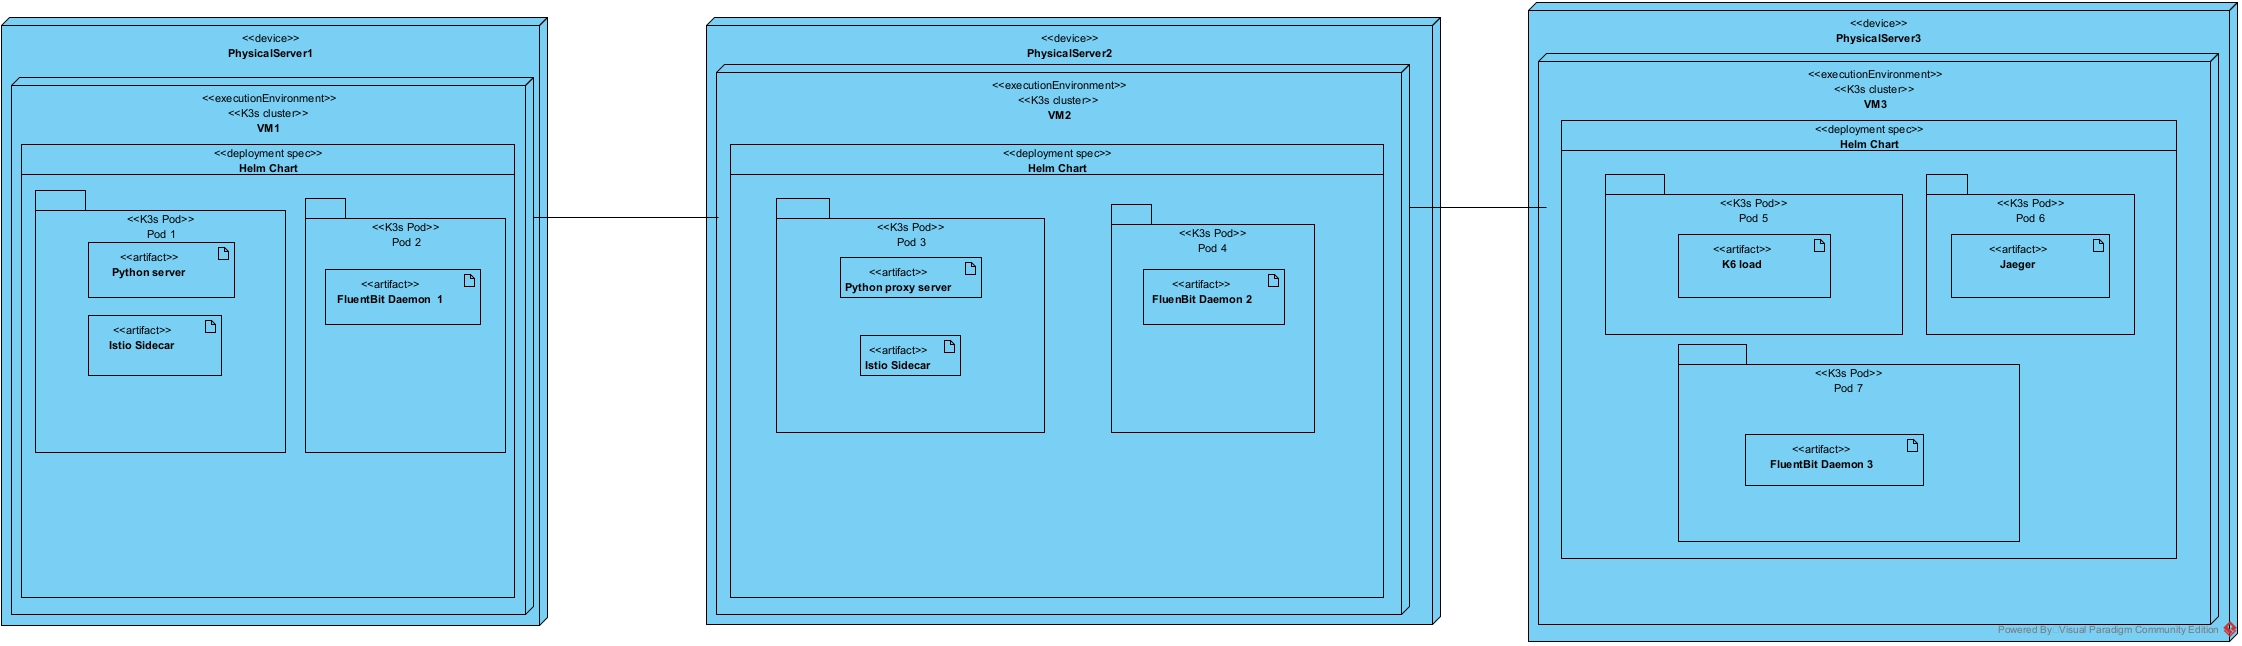
\includegraphics[width=\textheight, keepaspectratio]{./img/Deployment1.jpg}%
    }
    \caption{Диаграмма развертывания}
    \label{pic:deployment-diagram}
  \end{figure}
  

\dots



\section{Описание архитектуры системы с помощью диаграммы последовательности.}

\textbf{Аннотация.} \textit{Разработана модель коммуникаций, иллюстрирующая маршрутизацию запросов от инициирующего сервиса к конечному получателю. Приведено подробное описание последовательности обмена сообщениями между сервисами, демонстрирующее логику взаимодействия. Отражено, как в версии с использованием Istio трафик проходит через sidecar-компоненты, обеспечивая дополнительный контроль и безопасность. Приведено сравнение с самописной реализацией, где обмен сообщениями осуществляется напрямую без промежуточного proxy-слоя. Разработана последовательность вызовов, охватывающая все ключевые этапы обработки запросов в системе. Отражены различия в производительности и надежности между обеими реализациями коммуникации сервисов.}




% Команда \texorpdfstring необходима, чтобы программа просмотра PDF документов
% верно отображала текст формул в панели оглавления.
% При отсутствии команды \texorpdfstring там, где она необходима, LaTeX выводит
% предупреждение "Token not allowed in a PDF string"


\section{Выводы}

\textbf{Аннотация.} \textit{Получена достоверная модель системы, полностью отражающая архитектуру, которая остается лишь реализовать. Спроектированы основные программные модули, включая сервер, прокси-сервер и модуль генерации нагрузки k6. Учтены особенности физической инфраструктуры с разделением на физические серверы и виртуальные машины в кластере k3s. Отражена интеграция data collector для сбора и централизованной передачи логов и трейсов. Приведена схема автоматизированного развертывания с использованием Helm-чарта для управления микросервисами. Итоговый результат – надежная и полная инженерная модель, готовая к непосредственной реализации и проведению тестов.}

%%% Local Variables:
%%% TeX-engine: xetex
%%% eval: (setq-local TeX-master (concat "../" (seq-find (-cut string-match ".*-3-pz\.tex$" <>) (directory-files ".."))))
%%% End:
